\chapter{Introduction}

\hspace{5mm}The goal of this internship is to investigate the possibilities of GPGPU acceleration of numerical simulations and subroutines in use at the MEFD group. GPGPU acceleration leverages the computational power of the GPU to perform mathematical calculations that would otherwise be performed by the CPU.\vspace{4mm}

GPGPU is a hot topic at the moment, artificial intelligence and crypto currencies have taken a huge flight since they adapted to leverage the power of GPU's. As figure \ref{GPU chart 1} shows, the peak double precision FLOPS and memory bandwidth of GPU's has grown to be much larger than CPU's can provide.\vspace{4mm}

A reduction in runtime of numerical simulations has numerous advantages, the most obvious one is the ability to run larger simulations in the same runtime. Training of deep learning neural networks is a prime example. Much of the theory behind these applications was already available in the eighties, but the compute capabilities at the time where insufficient for practical use.\vspace{4mm}

The productivity of researchers also improves when they have access to increased computational power. It allows them to run more and better simulation, proving an enhanced insight into the results.

\begin{figure}[b!]
    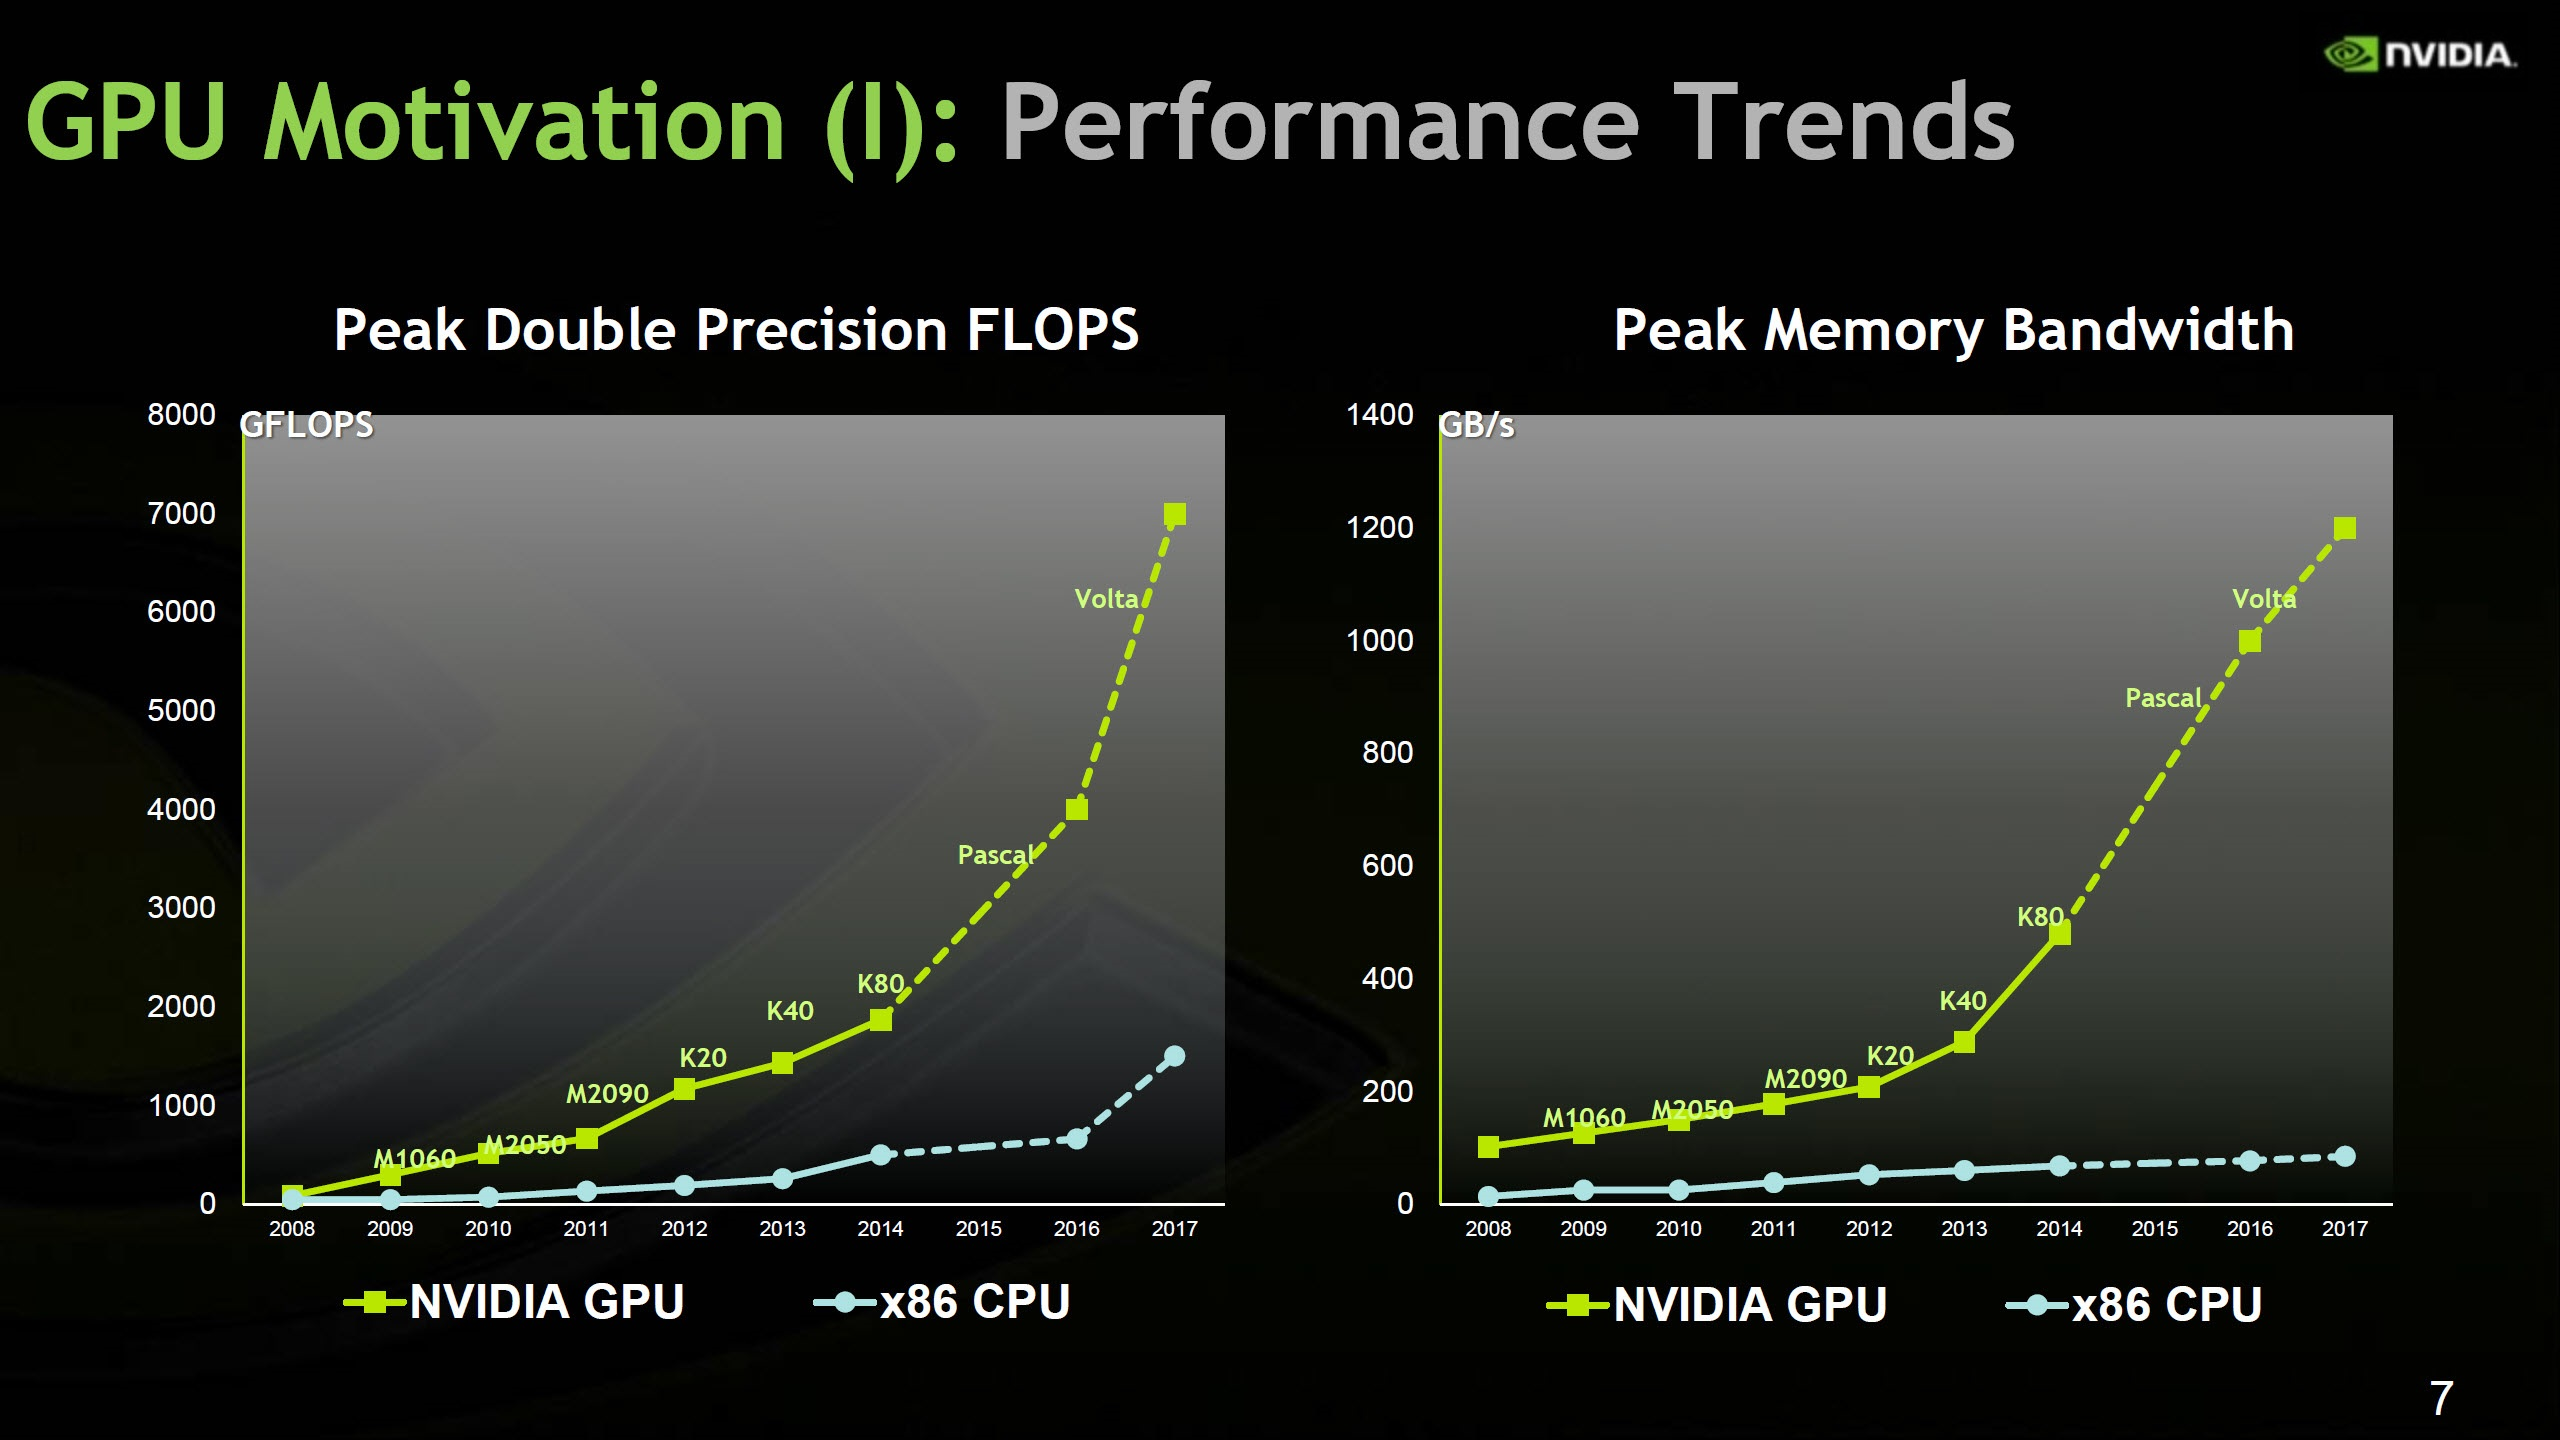
\includegraphics[width=0.85\linewidth]{figures/NVIDIA-Pascal-and-Volta-Compute-Performance.jpg}
    \centering
    \caption{Floating point and bandwidth performance comparison provided by NVIDIA.}
    \label{GPU chart 1}
\end{figure}

\newpage

\section{The MEFD group}

\hspace{5mm}The website of the Department of Mechanical Engineering faculty of the TU/e gives the following description of the MEFD group:\vspace{4mm}

\textit{The MEFD section focuses on the development, analysis and application of mathematical-physical models and advanced numerical techniques for multiscale flow problems in engineering applications, with particular emphasis on flow problems in the transitional molecular/continuum regime and auxiliary field interactions. The research in the section has an underpinning and methodological character, while maintaining a strong connection to applications in the high-tech industry and in other sections.} \autocite[]{tue_mefd_1}\vspace{4mm}

\noindent The work within the MEFD group can be roughly divided into 5 categories:

\begin{itemize}
    \item Research into various models of physics and engineering based problems.
    \item Investigating the mathematical aspects of the aforementioned models.
    \item Evaluating and enhancing discretization techniques and their relation to the models for numerical evaluation.
    \item Implementing the advancements in discretization methods into software (Nutils).
    \item Looking into various algorithms for solving the resulting linear system of equations.
\end{itemize}

The research within the MEFD group into iterative methods, stems from the problems encountered when using the more traditional direct solving techniques in their applications. Methods like LU decomposition can cause excessive run-times or residual errors, making them unsuitable in certain instances. A similar problem can arise when the simulations grow in size. The run-times can grow out of control when the amount of FLOP's required to evaluate the simulations scales badly with the dimensions of the simulation.\vspace{4mm}

The most obvious solution to this problem is to buy computers with increased computational power, but the recent movement towards GPGPU accelerated computers also requires a paradigm shift in programming techniques to leverage their capabilities to the fullest. The MEFD group has recently gained access to a GPGPU enabled server via the Rare Trans project of ASML in conjunction with the Energy Technology group, of which the MEFD group is a part. Its adoption for the simulations of the MEFD group is (at the time of writing) at an early stage.

\newpage

\section{The internship project}

\hspace{5mm}A lot of the numerical methods and simulations that are developed by the MEFD group are based on FEM (or related methods) and often require solving ill-conditioned block-sparse linear systems. These types of applications require relatively large amounts of RAM and double precision floating point data, resulting in additional difficulties when making the transition to GPGPU.\vspace{4mm}

This internship will lay the foundations for a discussion of these difficulties by providing the required background on floating point arithmetic, Amdahl's law and the workings of computers. A high level overview of computers and their history pertaining to scientific computing will be provided, followed by a description of the somewhat more low-level workings of a personal computer. \vspace{4mm}

The final chapter of this report will provide a brief summary of the topics of the master thesis project and their associated challenges.